\subsection{Klassische Softwarekomponenten}
\label{sec:2_Softwarekomponente_Klassisch}
\begin{quote}
\glqq The characteristic properties of a component are that it: \citereset \autocite[siehe][S. 35-38]{Szyperski.2002}\grqq
\begin{itemize}
\item is a unit of independent deployment
\item is a unit of third-party composition
\item has no (externally) observable state
\end{itemize}
\end{quote}

Dies ist die Definition einer Komponente von Clemens Szyperski aus dem Buch \glqq Component software: Beyond object-oriented programming\grqq\ \citereset \autocite[siehe][S. 35-38]{Szyperski.2002}.
Diese Definition bedarf hinsichtlich dieser Arbeit weiterer Erläuterung:
\begin{description}
\item[A component is a unit of independent deployment] \hfill \\
Dieser Punkt der Definition besitzt eine softwaretechnische Implikation. Damit eine Komponente \glqq independent deployable\grqq\ also unabhängig auslieferbar ist, muss sie auch so konzipiert beziehungsweise entwickelt werden. Sämtliche Funktionen der Komponente müssen vollständig unabhängig von der Verwendungsumgebung und von anderen Komponenten sein. Des Weiteren muss der Begriff \glqq independent deployable\grqq\ als Ganzes betrachtet werden, denn dies bedeutet, dass eine Komponente nicht partiell, sondern nur als Ganzes ausgeliefert wird.
\item[A component is a unit of third-party composition] \hfill \\
Hier wird der Begriff \glqq composable\grqq\ dahingehend verstanden, dass Komponenten zusammensetzbar sein sollen. In diesem Kontext bedeutet dies, dass eine Applikation aus mehreren Komponenten bestehen kann. Des Weiteren soll auch mit einer Komponente interagiert werden können, was einer klar definierten Schnittstelle bedarf. Nur mit Hilfe einer solchen Schnittstelle kann garantiert werden, dass die Komponente einerseits vollständig gekapselt von anderen Komponenten ist und andererseits mit der Umgebung interagieren kann. Dies erfordert demnach eine klare Spezifikation, was die Komponente einerseits erfordert und andererseits bereitstellt.
\item[A component has no (externally observable) state] \hfill \\
Eine Komponente sollte keinen externen \glqq observable\grqq\ (feststellbaren) Zustand haben. Die Originalkomponente darf nicht von Kopien ihrer selbst unterschiedlich sein. Dies garantiert, dass sämtliche Kopien einer Komponente nach außen hin \glqq gleich\grqq\ sind.
Eine mögliche Ausnahme dieser Regel wäre jedoch ein Attribut der Komponente, das nicht zu ihrer Funktionalität beiträgt. Ein Beispiel dafür wäre ein Attribut für die Zwischenspeicherung von Daten. Dieses Attribut hat keinerlei Auswirkung auf die Funktionalität der Komponente selbst, jedoch Auswirkung auf die Performanz dieser Komponente. Attribute dieser Art sind erlaubt.
\end{description}

Wenn eine Komponente mit Hilfe dieser Definition umgesetzt wird, gilt sie als vollständig wiederverwertbar.
Zugleich ergeben sich aus dieser Definition zwei Sichtweisen auf Komponenten. Zum einen die Sichtweise der Verwenderin beziehungsweise des Verwenders der Komponente (siehe Unterabbildung \ref{sfig:Komponente_Verwender} auf Seite \pageref{sfig:Komponente_Verwender}) und zum anderen die Sichtweise der Entwicklerin beziehungsweise des Entwicklers der Komponente (siehe Unterabbildung \ref{sfig:Komponente_Entwickler} auf Seite \pageref{sfig:Komponente_Entwickler}). Die Benutzerin und der Benutzer der Komponente können keine Aussagen darüber treffen, auf welcher Basis die die verwendete Komponente entwickelt wurde. Folglich kann die Implementierung als \glqq Black-Box\grqq\ für die Verwenderin beziehungsweise den Verwender gesehen werden. Die Entwicklerin beziehungsweise der Entwickler hingegen hat vollständiges Wissen über den Aufbau und das Verhalten der Komponente.

\begin{figure}[h]
  \centering
  \subfloat[Software-Komponente aus der Sichtweise des Verwenders]{
    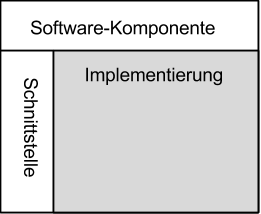
\includegraphics[height=5.0cm]{images/Software-Komponente-Verwender.png}
    \label{sfig:Komponente_Verwender}
  }
  \qquad
  \subfloat[Software-Komponente aus der Sichtweise des Entwicklers]{
    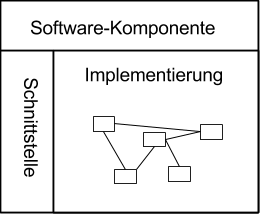
\includegraphics[height=5.0cm]{images/Software-Komponente-Entwickler.png}
    \label{sfig:Komponente_Entwickler}
  }
  \caption[
    Software-Komponente aus unterschiedlichen Sichtweisen
  ]{
    Software-Komponente aus unterschiedlichen Sichtweisen
  }
  \label{fig:Komponente_Sichtweise}
\end{figure}

In vielen aktuellen Ansätzen sind Komponenten eine große Einheit mit genau einer Instanz in einem System. Beispielsweise könnte ein Datenbankserver eine Komponente darstellen. Oftmals wird der Datenbankserver im Zusammenhang mit der Datenbank als Modul mit einem feststellbaren Zustand angesehen. Dahingehend ist der Datenbankserver ein Beispiel für eine Komponente und die Datenbank ein Beispiel für das Objekt, das von der Komponente verwaltet wird. Es ist wichtig zwischen dem Komponentenkonzept und dem Objektkonzept zu differenzieren, da das Komponentenkonzept keinen Gebrauch von Zuständen von Objekten fördert \citereset \autocite[siehe][S. 35-38]{Szyperski.2002}.

Eine Softwarearchitektur ist die zentrale Grundlage einer skalierbaren Softwaretechnologie und ist für komponentenbasierte Systeme von größter Bedeutung. Nur da, wo eine Gesamtarchitektur mit Wartbarkeit definiert ist, finden Komponenten die Grundlage, die sie benötigen.